% Session 1 -- one Hamiltonian, three broken symmetries.
% Placement: sec. "The general interacting Hamiltonian", alongside the enumerated list.
% Rendered by figures/blender/s01f03_threechannels.py, labels in figures/overlays/s01f03_threechannels.tex.
\begin{aqmfigure}{fig:s01:channels}{One Hamiltonian and three ordered states. The same generic
interacting Hamiltonian (1.5), on the left, where the glow is the interaction between two electrons
on neighboring sites, is decoupled with three different bilinear expectation values. This gives a
charge density wave, a magnet or a superconductor, each breaking a different symmetry. The charge is
drawn as columns of alternating height, the spin as alternating arrows, and the electrons bound in
pairs as two balls inside one capsule. These three branches are the structure on which the rest of
the course is organized.}
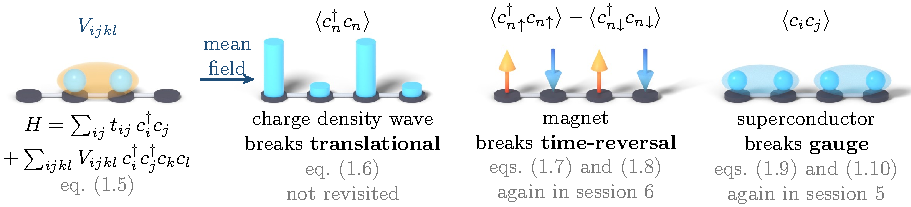
\includegraphics{figures/pdf/s01f03_threechannels.pdf}
\end{aqmfigure}
